\documentclass[11pt,a4paper]{article}
\usepackage[T1]{fontenc}
\usepackage[utf8]{inputenc}
\usepackage[spanish,es-noshorthands,es-nolists,es-noquoting]{babel}
\usepackage{mathptmx}
\usepackage{amsmath,amssymb,textcomp}
\usepackage[a4paper,top=2.5cm,bottom=2.3cm,left=2.5cm,right=2.5cm]{geometry}
\usepackage{xcolor}
\usepackage{calc}
\usepackage{longtable,booktabs,array}
\usepackage{etoolbox}
\makeatletter\patchcmd\longtable{\par}{\if@noskipsec\mbox{}\fi\par}{}{}\makeatother
\usepackage{graphicx}
\usepackage{float}
\usepackage[font=small,it]{caption}
\usepackage{enumitem}
\usepackage{microtype}
\usepackage{titlesec}
\usepackage{fancyhdr}
\usepackage{xurl}
\usepackage[hidelinks]{hyperref}
\urlstyle{same}

\DeclareUnicodeCharacter{2248}{$\approx$}
\DeclareUnicodeCharacter{2212}{$-$}
\DeclareUnicodeCharacter{00B1}{$\pm$}
\DeclareUnicodeCharacter{00B2}{\textsuperscript{2}}
\DeclareUnicodeCharacter{00B7}{\textperiodcentered}
\DeclareUnicodeCharacter{00A7}{\S}

\setlength{\parindent}{1.3em}
\setlength{\parskip}{0.35ex plus 0.2ex}
\linespread{1.04}
\setlist{nosep,leftmargin=1.4em,topsep=0.4ex,itemsep=0.3ex}
\captionsetup{skip=4pt}

\titleformat{\section}{\normalfont\large\bfseries}{}{0pt}{}
\titleformat{\subsection}{\normalfont\normalsize\bfseries}{}{0pt}{}
\titlespacing*{\section}{0pt}{12pt plus 2pt}{5pt}
\titlespacing*{\subsection}{0pt}{9pt plus 2pt}{3pt}

\pagestyle{fancy}\fancyhf{}
\renewcommand{\headrulewidth}{0.4pt}
\fancyhead[L]{\footnotesize Home Credit · Trabajo Práctico}
\fancyhead[R]{\footnotesize Machine Learning · MiM + Analytics}
\fancyfoot[C]{\footnotesize\thepage}

\providecommand{\tightlist}{\setlength{\itemsep}{0pt}\setlength{\parskip}{0pt}}

\begin{document}
\begin{titlepage}
\centering
\thispagestyle{empty}
\vspace*{2.2cm}


\includegraphics[width=0.46\textwidth]{logo.png}

\vspace{1.1cm}
{\normalsize MiM + Analytics · 2026}\\[0.3em]
{\normalsize Machine Learning}

\vspace{1.9cm}
\rule{\textwidth}{0.5pt}\\[0.9em]
{\LARGE\bfseries Trabajo Práctico}\\[0.9em]
{\large Aplicaciones de Aprendizaje Automático}\\[0.5em]
{\normalsize Home Credit Default Risk · Valuación de vivienda en Argentina}\\[0.9em]
\rule{\textwidth}{0.5pt}

\vspace{2.4cm}
{\bfseries Integrantes}\\[0.6em]
Albertina Ferreyra\\
María Florencia Grimaldi\\
Lucía Koopmann

\vfill
Repositorio: \url{https://github.com/mfgrimaldi/tp1-homecredit}\\[0.8em]
Fecha de entrega: 4 de octubre de 2026
\end{titlepage}

\section*{Introducción}
La \textbf{Parte 1} resuelve la competencia Home Credit Default Risk: predecir la probabilidad de que un cliente no pague su préstamo, optimizando ROC AUC. Partimos de una regresión logística sobre la tabla principal (AUC 0,7448) y llegamos a un LightGBM con variables construidas desde las cinco tablas y optimización de hiperparámetros (AUC 0,7847 en validación cruzada; 0,7824 en Kaggle Private). El salto vino de los datos, no del modelo: las variables nuevas aportaron +0,018, el cambio de modelo +0,020 y el tuning +0,002.

La \textbf{Parte 2} formula un problema propio sobre datos abiertos de Properati: estimar el valor de mercado de una vivienda residencial en Argentina para que una inversora priorice qué propiedades visitar. Un modelo out-of-the-box reduce el error un 57\% contra el baseline (MAPE 24,9\% contra 59,2\%), lo que confirma que hay señal; el análisis de factibilidad muestra que los límites no son del modelo sino de los datos y de su vigencia en el tiempo.

Todo el código, los resultados intermedios y las submissions están en el repositorio del grupo: \url{https://github.com/mfgrimaldi/tp1-homecredit}.

\section*{Parte 1 · Home Credit Default Risk}

\subsection*{1.1 Problema y datos}

El objetivo es predecir la probabilidad de que un cliente tenga dificultades de pago (\emph{TARGET = 1}). La métrica de la competencia es ROC AUC: la probabilidad de que el modelo asigne más riesgo a un cliente que no pagó que a uno que sí pagó, tomados al azar. La clase positiva es minoritaria (8,07\%), por eso se usa una métrica de ranking y folds estratificados.

\begin{longtable}[]{@{}
  >{\raggedright\arraybackslash}p{(\columnwidth - 4\tabcolsep) * \real{0.2800}}
  >{\raggedright\arraybackslash}p{(\columnwidth - 4\tabcolsep) * \real{0.5201}}
  >{\raggedright\arraybackslash}p{(\columnwidth - 4\tabcolsep) * \real{0.2000}}@{}}
\toprule\noalign{}
\begin{minipage}[b]{\linewidth}\raggedright
\textbf{Archivo}
\end{minipage} & \begin{minipage}[b]{\linewidth}\raggedright
\textbf{Contenido}
\end{minipage} & \begin{minipage}[b]{\linewidth}\raggedright
\textbf{Filas}
\end{minipage} \\
\midrule\noalign{}
\endhead
\bottomrule\noalign{}
\endlastfoot
application\_\allowbreak{}train / test & Una fila por préstamo solicitado (122 columnas) & 307.511 / 48.744 \\
bureau & Créditos del cliente en otras entidades & 1,7 M \\
previous\_\allowbreak{}application & Solicitudes anteriores en Home Credit & 1,7 M \\
installments\_\allowbreak{}payments & Pagos de cuotas de créditos anteriores & 13,6 M \\
bureau\_\allowbreak{}balance & Estado mes a mes de cada crédito del bureau & 27,3 M \\
POS\_\allowbreak{}CASH, credit\_\allowbreak{}card & Historiales mensuales (no utilizados) & --- \\
\end{longtable}

\subsection*{1.2 Esquema de validación}

Validación cruzada estratificada de 5 folds con semilla fija (42). Cada préstamo tiene asignado su fold en un archivo versionado en git, de modo que todos los experimentos del grupo se comparan sobre exactamente la misma partición. Cada fold conserva la tasa de default (≈8,07\%) y contiene unos 61.500 préstamos.

\begin{itemize}
\item
  Reportamos AUC out-of-fold: cada préstamo se predice con el modelo que no lo vio al entrenar.
\item
  Todo el preprocesamiento (imputación, escalado, codificación) va dentro de un Pipeline, de modo que se ajusta solo con el train de cada fold y no hay fuga de información.
\item
  La predicción de test es el promedio de los cinco modelos, uno por fold.
\item
  Chequeo contra Kaggle: la diferencia entre validación y Kaggle fue de 0,011 con la logística y de 0,002 con el modelo final, lo que respalda usar la validación para elegir modelos.
\end{itemize}

\textbf{Advertencia metodológica:} el AUC de 0,7847 es el mejor de 30 pruebas de optimización evaluadas sobre esos mismos folds, por lo que está algo sobreestimado como estimación del desempeño futuro. El score de Kaggle, que proviene de datos no usados en ninguna etapa, lo confirma con una diferencia de 0,002.

\subsection*{1.3 Preprocesamiento y feature engineering}

Sobre la tabla principal construimos variables que capturan relaciones económicas que las columnas originales no expresan de forma directa:

\begin{longtable}[]{@{}
  >{\raggedright\arraybackslash}p{(\columnwidth - 4\tabcolsep) * \real{0.3000}}
  >{\raggedright\arraybackslash}p{(\columnwidth - 4\tabcolsep) * \real{0.2800}}
  >{\raggedright\arraybackslash}p{(\columnwidth - 4\tabcolsep) * \real{0.4200}}@{}}
\toprule\noalign{}
\begin{minipage}[b]{\linewidth}\raggedright
\textbf{Variable}
\end{minipage} & \begin{minipage}[b]{\linewidth}\raggedright
\textbf{Cálculo}
\end{minipage} & \begin{minipage}[b]{\linewidth}\raggedright
\textbf{Qué captura}
\end{minipage} \\
\midrule\noalign{}
\endhead
\bottomrule\noalign{}
\endlastfoot
CREDIT\_\allowbreak{}INCOME\_\allowbreak{}RATIO & préstamo / ingreso & Cuántos ingresos anuales debe \\
ANNUITY\_\allowbreak{}INCOME\_\allowbreak{}RATIO & cuota / ingreso & Qué parte del ingreso se va en la cuota \\
CREDIT\_\allowbreak{}TERM & cuota / préstamo & ≈ 1/plazo: cuota alta implica plazo corto \\
GOODS\_\allowbreak{}CREDIT\_\allowbreak{}RATIO & precio del bien / préstamo & Menor a 1 si financia más que el bien \\
INCOME\_\allowbreak{}PER\_\allowbreak{}PERSON & ingreso / miembros del hogar & Ingreso disponible por persona \\
AGE\_\allowbreak{}YEARS, EMPLOYED\_\allowbreak{}AGE\_\allowbreak{}RATIO & edad; días trabajados / días de vida & Edad y estabilidad laboral \\
DAYS\_\allowbreak{}EMPLOYED\_\allowbreak{}ANOM & marca DAYS\_\allowbreak{}EMPLOYED = 365.243 & Valor centinela en el 18\% de las filas; el original pasa a nulo \\
EXT\_\allowbreak{}SOURCE\_\allowbreak{}MEAN/\allowbreak MIN/\allowbreak MAX/\allowbreak STD & resúmenes de los 3 scores externos & EXT\_\allowbreak{}SOURCE\_\allowbreak{}1 falta en 56\%: el resumen aprovecha los disponibles \\
DOCS\_\allowbreak{}COUNT & suma de FLAG\_\allowbreak{}DOCUMENT\_\allowbreak{}* & Documentos presentados \\
\end{longtable}

Las tablas auxiliares tienen varias filas por cliente, así que se resumen a una fila por cliente agregando por SK\_\allowbreak{}ID\_\allowbreak{}CURR antes de unirlas. Ninguna agregación usa la variable objetivo, por lo que no introducen fuga de información:

\begin{itemize}
\item
  bureau: cantidad de créditos y activos, deuda total, deuda sobre monto, montos vencidos, máximo atraso, antigüedad del crédito más reciente, prórrogas.
\item
  previous\_\allowbreak{}application: cantidad de pedidos, porcentaje rechazado y aprobado, pedido sobre otorgado, monto y cuota media, plazo medio, días desde el último pedido.
\item
  installments\_\allowbreak{}payments: porcentaje de cuotas pagadas tarde, días de atraso medio y máximo, porcentaje de cuotas pagadas de menos, ratio pagado sobre adeudado.
\end{itemize}

Medido con la misma logística y los mismos folds, agregando un bloque a la vez:

\begin{longtable}[]{@{}
  >{\raggedright\arraybackslash}p{(\columnwidth - 6\tabcolsep) * \real{0.4600}}
  >{\raggedright\arraybackslash}p{(\columnwidth - 6\tabcolsep) * \real{0.1800}}
  >{\raggedright\arraybackslash}p{(\columnwidth - 6\tabcolsep) * \real{0.1800}}
  >{\raggedright\arraybackslash}p{(\columnwidth - 6\tabcolsep) * \real{0.1800}}@{}}
\toprule\noalign{}
\begin{minipage}[b]{\linewidth}\raggedright
\textbf{Paso}
\end{minipage} & \begin{minipage}[b]{\linewidth}\raggedright
\textbf{Variables}
\end{minipage} & \begin{minipage}[b]{\linewidth}\raggedright
\textbf{AUC}
\end{minipage} & \begin{minipage}[b]{\linewidth}\raggedright
\textbf{Mejora}
\end{minipage} \\
\midrule\noalign{}
\endhead
\bottomrule\noalign{}
\endlastfoot
0. Baseline sin feature engineering & 120 & 0,7448 & --- \\
1. + ratios de application & 134 & 0,7495 & +0,0047 \\
2. + bureau & 146 & 0,7531 & +0,0036 \\
3. + previous\_\allowbreak{}application & 154 & 0,7587 & +0,0056 \\
4. + installments\_\allowbreak{}payments & 160 & 0,7628 & +0,0041 \\
\end{longtable}

\begin{figure}[H]
\centering
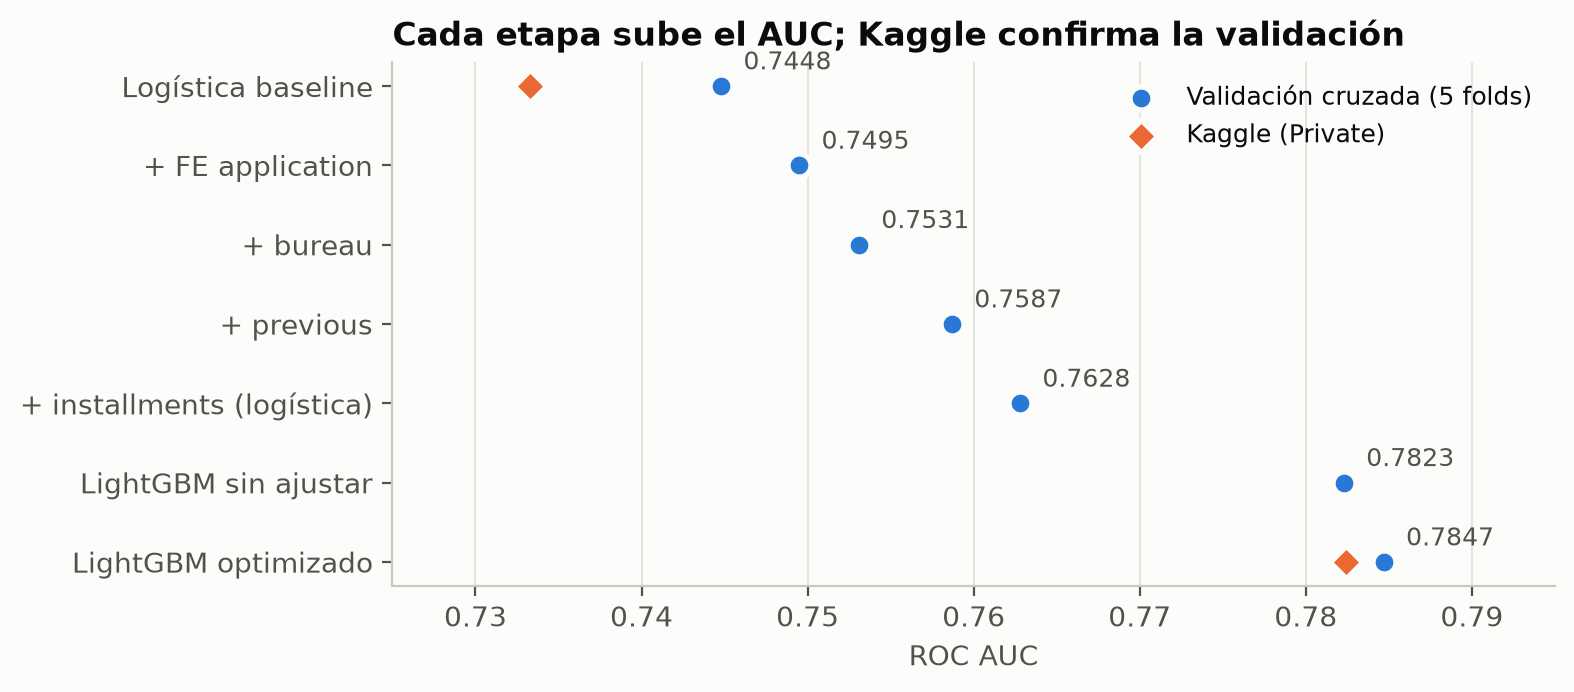
\includegraphics[width=0.90\linewidth]{media/figura1_auc_por_etapa.png}
\caption*{Figura 1. AUC por etapa (validación cruzada) y score de Kaggle Private de las dos submissions.}
\end{figure}\textbf{Un bloque adicional, medido y descartado.} Los bloques anteriores dejan afuera bureau\_\allowbreak{}balance, el estado mes a mes de cada crédito reportado al Credit Bureau y, con 27,3 millones de filas, la tabla más grande del conjunto. Como tiene una fila por crédito y por mes, resumirla exige una agregación en dos niveles: primero el historial mensual de cada crédito y después los créditos de cada cliente. Construimos así 78 variables, entre ellas la proporción de meses en mora de cada crédito, el peor tramo de atraso alcanzado y los meses en mora del último año, que es información que los agregados simples de bureau no distinguen de una mora antigua.

\textbf{Resultado de la comparación.} Medido contra el bloque de bureau ya incorporado, con los mismos folds y el mismo LightGBM optimizado, el AUC out-of-fold pasa de 0,7846 a 0,7867, con mejora en los cinco folds (diferencia media de 0,0021 y desvío de 0,0009). Usar las dos versiones de bureau juntas no aporta nada adicional (0,7867), señal de que miden lo mismo. Aun así mantuvimos el modelo final sin este bloque: la mejora es del mismo orden que el sesgo optimista ya señalado sobre el 0,7847, que es el mejor de 30 pruebas evaluadas sobre estos mismos folds, y adoptarlo implicaba rehacer también la interpretabilidad de la sección 1.7. El experimento deja una conclusión de rendimiento decreciente: el historial mensual representa el 94\% de las filas de las tablas del bureau y aporta 0,002 de AUC, porque la señal ya estaba casi toda capturada por el resumen a nivel crédito. El código y la comparación completa quedan en el repositorio (src/features\_\allowbreak{}bureau.py y resultados\_\allowbreak{}bureau/).

\subsection*{1.4 Codificación de variables categóricas}

Para la logística usamos one-hot, agrupando las categorías con menos del 1\% de las filas para no crear columnas ruidosas; las numéricas se imputan por mediana y se estandarizan, porque la regularización lo requiere. Para LightGBM comparamos one-hot contra su manejo nativo de categóricas: 0,7827 ± 0,0036 contra 0,7823 ± 0,0030. La diferencia (0,0004) es mucho menor que la variación entre folds, así que es ruido; elegimos la codificación nativa por ser más simple y rápida.

\subsection*{1.5 Modelos y optimización}

\begin{itemize}
\item
  Regresión logística (baseline): interpretable y rápida, pero solo capta relaciones lineales en log-odds.
\item
  LightGBM: suma muchos árboles chicos, cada uno corrigiendo los errores de los anteriores; capta no linealidades e interacciones sin programarlas.
\end{itemize}

La optimización se hizo con Optuna (algoritmo TPE), que propone cada combinación mirando cuáles dieron mejor AUC y por eso necesita menos pruebas que una grilla. Cada combinación se evaluó con los mismos 5 folds, con learning rate 0,05 y early stopping, de modo que la cantidad de árboles también se optimiza: 30 pruebas, unos 55 minutos.

\begin{longtable}[]{@{}
  >{\raggedright\arraybackslash}p{(\columnwidth - 4\tabcolsep) * \real{0.4400}}
  >{\raggedright\arraybackslash}p{(\columnwidth - 4\tabcolsep) * \real{0.3000}}
  >{\raggedright\arraybackslash}p{(\columnwidth - 4\tabcolsep) * \real{0.2600}}@{}}
\toprule\noalign{}
\begin{minipage}[b]{\linewidth}\raggedright
\textbf{Hiperparámetro}
\end{minipage} & \begin{minipage}[b]{\linewidth}\raggedright
\textbf{Rango explorado}
\end{minipage} & \begin{minipage}[b]{\linewidth}\raggedright
\textbf{Mejor valor}
\end{minipage} \\
\midrule\noalign{}
\endhead
\bottomrule\noalign{}
\endlastfoot
num\_\allowbreak{}leaves (hojas por árbol) & 8 -- 128 (log) & 9 \\
min\_\allowbreak{}child\_\allowbreak{}samples & 20 -- 500 (log) & 47 \\
subsample (filas por árbol) & 0,5 -- 1,0 & ≈ 1,0 \\
colsample\_\allowbreak{}bytree (columnas por árbol) & 0,1 -- 0,8 & 0,34 \\
reg\_\allowbreak{}lambda (L2) & 0,001 -- 30 (log) & 6,8 \\
reg\_\allowbreak{}alpha (L1) & 0,001 -- 10 (log) & 7,6 \\
Cantidad de árboles & early stopping & 2.357 con lr 0,05 \\
\end{longtable}

Para el modelo final bajamos el learning rate a 0,02 y escalamos los árboles en la misma proporción (5.892), lo que dio 0,7847 ± 0,0032 (+0,0024 contra los valores por defecto). La lectura es que el mejor modelo son muchos árboles chicos (9 hojas), que ven un tercio de las variables cada uno y están muy regularizados: con datos ruidosos conviene sumar muchas reglas simples antes que confiar en pocas reglas complejas.

\subsection*{1.6 Resultados en Kaggle}

\begin{longtable}[]{@{}
  >{\raggedright\arraybackslash}p{(\columnwidth - 6\tabcolsep) * \real{0.4600}}
  >{\raggedright\arraybackslash}p{(\columnwidth - 6\tabcolsep) * \real{0.1800}}
  >{\raggedright\arraybackslash}p{(\columnwidth - 6\tabcolsep) * \real{0.1800}}
  >{\raggedright\arraybackslash}p{(\columnwidth - 6\tabcolsep) * \real{0.1800}}@{}}
\toprule\noalign{}
\begin{minipage}[b]{\linewidth}\raggedright
\textbf{Submission}
\end{minipage} & \begin{minipage}[b]{\linewidth}\raggedright
\textbf{CV}
\end{minipage} & \begin{minipage}[b]{\linewidth}\raggedright
\textbf{Private}
\end{minipage} & \begin{minipage}[b]{\linewidth}\raggedright
\textbf{Public}
\end{minipage} \\
\midrule\noalign{}
\endhead
\bottomrule\noalign{}
\endlastfoot
Logística baseline & 0,7448 & 0,7333 & 0,7368 \\
LightGBM + FE + Optuna & 0,7847 & 0,7824 & 0,7869 \\
\end{longtable}

Como referencia, el primer puesto de la competencia obtuvo aproximadamente 0,806 (Private) con cientos de variables y ensambles de muchos modelos.

\subsection*{1.7 Interpretabilidad}

Entrenamos el LightGBM final con todo el conjunto de entrenamiento y aplicamos dos técnicas. La importancia por ganancia mide cuánto mejoró el modelo en los cortes que usan cada variable: dice qué variables usa más, pero no en qué dirección empujan. Los valores SHAP indican, para cada cliente, cuánto suma o resta cada variable respecto del promedio, en escala log-odds: dicen qué pesa y hacia dónde. Se calcularon sobre una muestra de 10.000 clientes.

\begin{figure}[H]
\centering
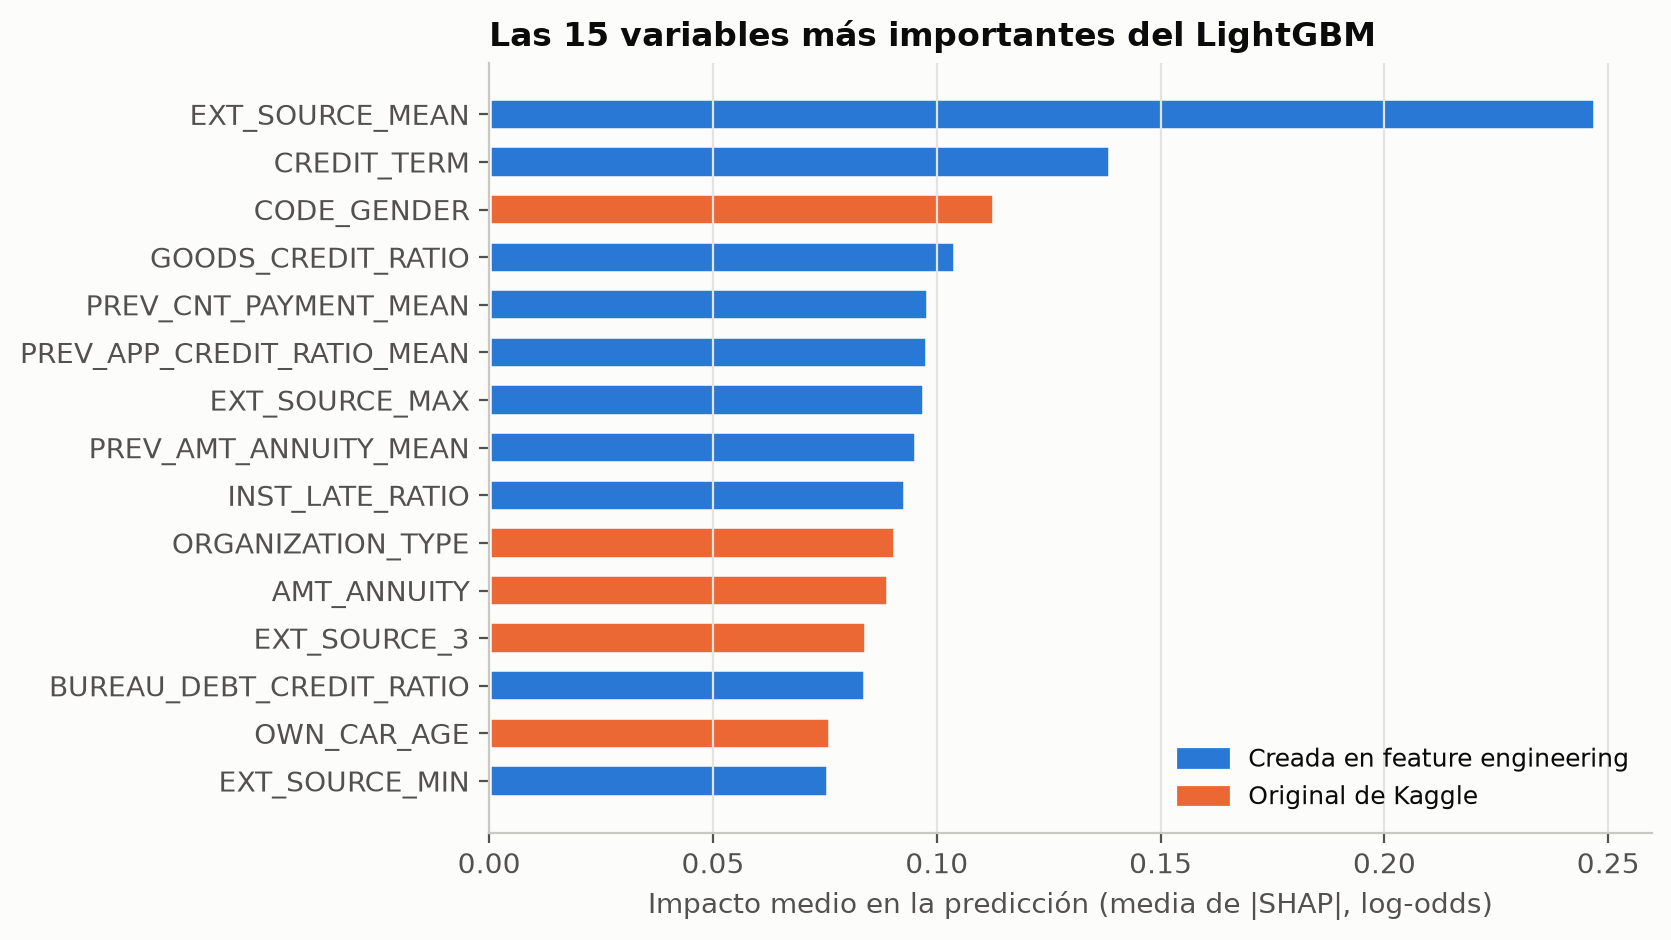
\includegraphics[width=0.83\linewidth]{media/figura2_shap_importancia.png}
\caption*{Figura 2. Importancia global (media del valor absoluto de SHAP). En azul, las variables creadas en el feature engineering: 10 de las 15 principales.}
\end{figure}\begin{itemize}
\item
  EXT\_\allowbreak{}SOURCE\_\allowbreak{}MEAN es la variable más importante: el 10\% con promedio más bajo suma +0,52 log-odds de riesgo y el 10\% más alto resta 0,44, con una relación casi lineal y decreciente.
\item
  CREDIT\_\allowbreak{}TERM (cuota sobre préstamo) es muy no lineal, con saltos según el plazo del producto: los préstamos de plazo corto tienen menos riesgo. Esta forma explica por qué los árboles superan a la logística.
\item
  Historial de pagos: sin cuotas pagadas tarde el efecto es −0,09; con más del 24\% pagadas tarde, +0,22. En otras entidades, el riesgo es plano hasta deber cerca del 40\% del monto y desde ahí sube de forma sostenida.
\item
  Financiar más que el bien y haber tomado plazos largos antes aumentan el riesgo; por tipo de organización, los empleados de escuelas presentan el menor riesgo y los autónomos el mayor.
\end{itemize}

\begin{figure}[H]
\centering
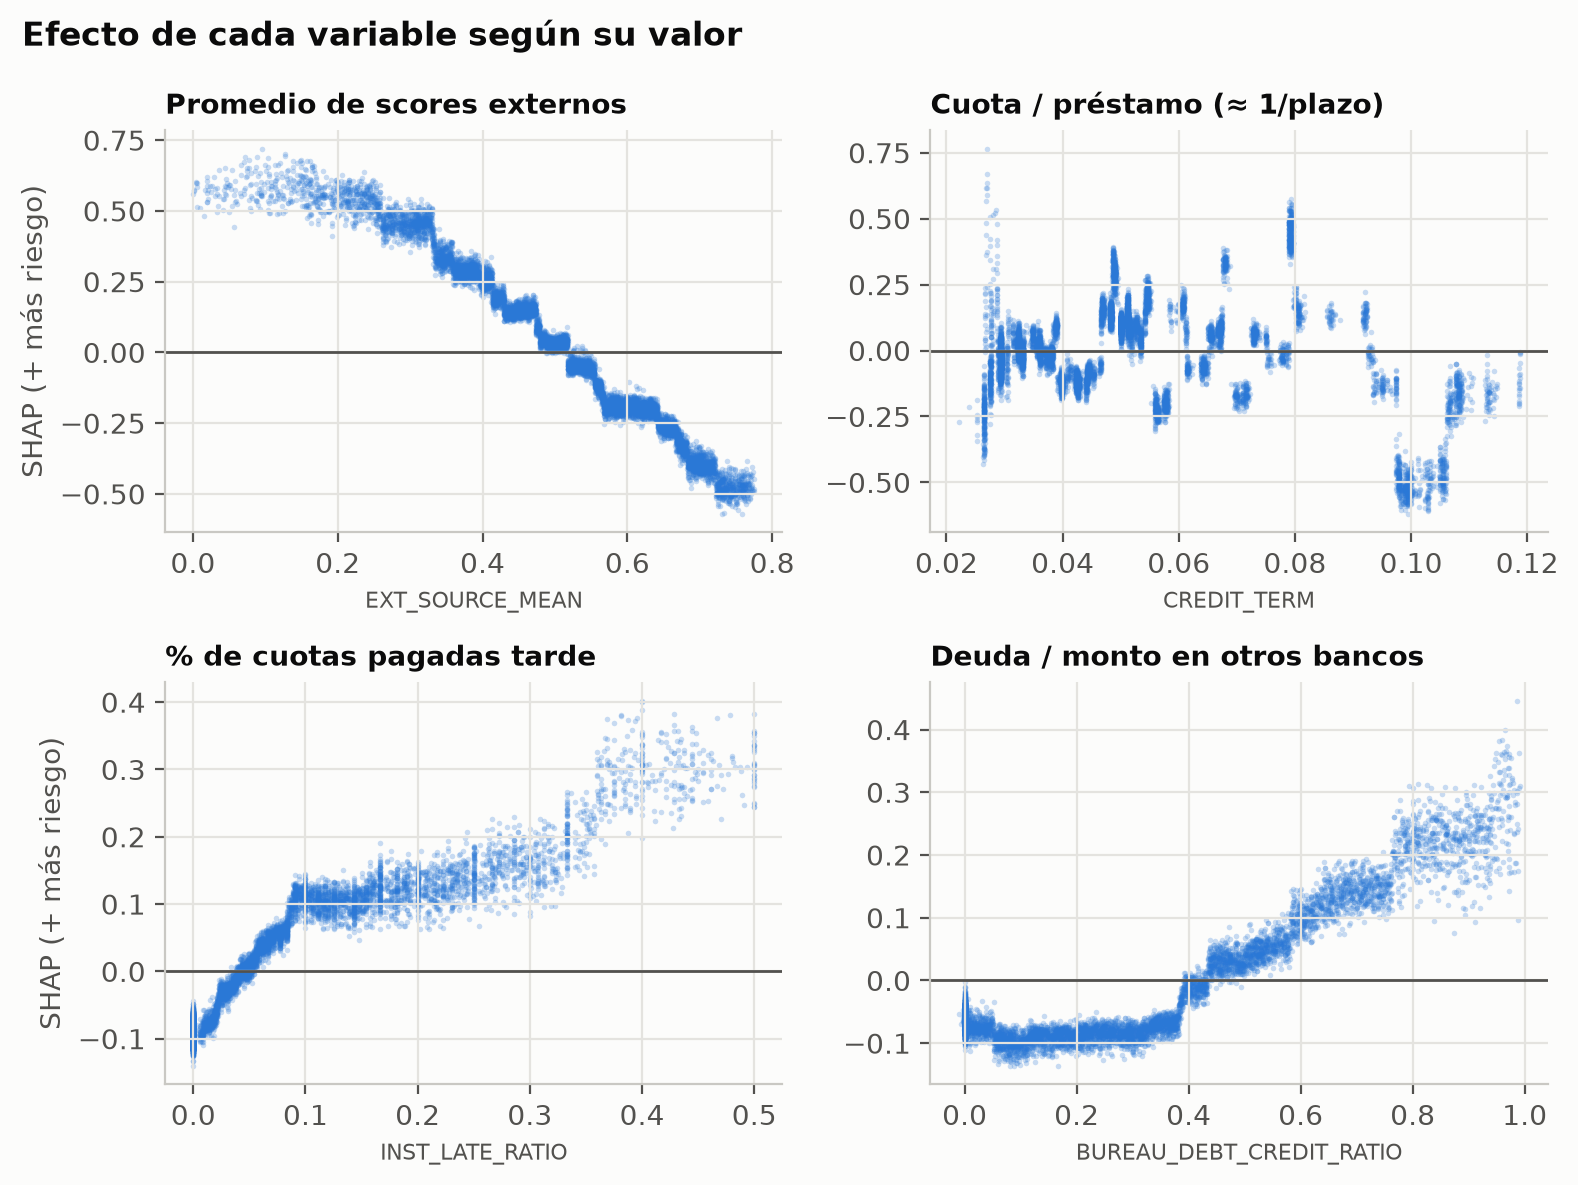
\includegraphics[width=0.89\linewidth]{media/figura3_shap_dependencia.png}
\caption*{Figura 3. Efecto SHAP según el valor de la variable, para cuatro variables creadas en el feature engineering.}
\end{figure}\subsection*{1.8 Discusión}

\textbf{Uso del género.} CODE\_\allowbreak{}GENDER es la tercera variable más importante del modelo: ser hombre suma +0,16 log-odds y ser mujer resta 0,09. Es predictivo, pero usar el género para decidir el otorgamiento de un crédito constituye discriminación por una característica protegida y está regulado en muchas jurisdicciones. Que una variable mejore la métrica no la vuelve legítima: la decisión de incluirla es normativa, no estadística. Dejamos pendiente medir cuánto AUC se pierde al excluirla, que es el dato que permitiría discutir el costo de esa decisión.

\textbf{Ganancia y SHAP no coinciden.} ORGANIZATION\_\allowbreak{}TYPE aparece cuarta por ganancia y décima por SHAP. Las variables categóricas con muchos valores se usan en muchos cortes e inflan la ganancia, por lo que SHAP es más confiable para comparar importancias entre variables de distinta naturaleza.

\textbf{Un efecto contraintuitivo.} Los clientes a quienes se les otorgó más de lo que pidieron presentan mayor riesgo. Probablemente refleje seguros u otros extras financiados dentro del préstamo, más que una decisión del cliente; queda como hipótesis a verificar.

\section*{Parte 2 · Valuación de vivienda y detección de oportunidades}

\subsection*{2.1 El problema de negocio}

Una inversora que compra propiedades para refaccionar y revender debe decidir, sobre un flujo constante de avisos nuevos, cuáles vale la pena visitar. Hoy esa selección se hace a ojo, comparando mentalmente con propiedades parecidas de la zona, y el recurso escaso no es el capital sino el tiempo de visita.

El modelo estima el valor de mercado de una vivienda a partir de sus características y su ubicación. La propiedad publicada muy por debajo de ese valor estimado es candidata a oportunidad. Al decidir, la inversora cuenta con lo que el propio aviso informa: superficie, ambientes, baños, tipo de propiedad, barrio y coordenadas, es decir, toda la información necesaria está disponible en el momento de la decisión.

\textbf{Supuesto central, y límite del enfoque:} un precio por debajo del estimado puede señalar una oportunidad o puede reflejar un defecto que el modelo no observa (estado de conservación, problemas de escritura, orientación, ruido). El modelo no distingue ``barata'' de ``barata por algo''. Por eso su salida prioriza visitas; no reemplaza la visita.

Qué error duele más: sobreestimar el valor lleva a pagar de más, con pérdida económica directa; subestimarlo hace perder una oportunidad, con un costo de oportunidad menor. La asimetría es relevante porque ninguna de las dos métricas que reportamos la captura, como se discute más abajo.

\subsection*{2.2 Datos y alcance}

El dataset de Properati contiene 992.192 avisos (25 columnas, julio 2019 a julio 2020). Los recortes definen el alcance del modelo y cada uno responde a una razón distinta:

\begin{longtable}[]{@{}
  >{\raggedright\arraybackslash}p{(\columnwidth - 4\tabcolsep) * \real{0.3300}}
  >{\raggedright\arraybackslash}p{(\columnwidth - 4\tabcolsep) * \real{0.4700}}
  >{\raggedright\arraybackslash}p{(\columnwidth - 4\tabcolsep) * \real{0.2000}}@{}}
\toprule\noalign{}
\begin{minipage}[b]{\linewidth}\raggedright
\textbf{Recorte}
\end{minipage} & \begin{minipage}[b]{\linewidth}\raggedright
\textbf{Razón}
\end{minipage} & \begin{minipage}[b]{\linewidth}\raggedright
\textbf{Filas}
\end{minipage} \\
\midrule\noalign{}
\endhead
\bottomrule\noalign{}
\endlastfoot
Dataset completo & --- & 992.192 \\
Argentina y operación de venta & El alquiler tiene precio mensual: otra unidad & 750.694 \\
Solo precios en dólares & Convertir pesos exigiría el tipo de cambio de cada fecha & 685.465 \\
Casa, Departamento y PH & Lotes y cocheras son otro producto, con otra lógica de precio & 383.118 \\
Precio entre 20.000 y 1.000.000 & Alcance: vivienda residencial, ni irrisorias ni suntuarias & 376.281 \\
Con superficie informada & Sin superficie no hay tasación posible & 237.686 \\
\end{longtable}

La pérdida mayor no es de alcance sino de calidad: \textbf{el 37\% de las viviendas no tiene cargada ninguna superficie}, ni total ni cubierta. Para las que informan al menos una, usamos la superficie total y, cuando falta, la cubierta. También faltan baños (6,6\%), ambientes (20,8\%) y coordenadas (12,5\%); el modelo elegido maneja nulos de forma nativa, así que esas filas se conservan.

\subsection*{2.3 Validación: partición temporal}

Dividimos por fecha de publicación y no al azar: se entrena con los avisos anteriores al 1 de abril de 2020 (178.809) y se evalúa con los posteriores (58.877). Es la forma en que el modelo se usaría en la realidad, donde siempre se predice sobre avisos nuevos con un modelo entrenado en el pasado. Una partición aleatoria mezclaría avisos del futuro en el entrenamiento y daría una estimación optimista. El corte coincide con el inicio de la pandemia, lo que vuelve la evaluación más exigente y, como se ve en §2.6, informativa.

\subsection*{2.4 Baseline y prototipo}

El baseline es el modelo más simple que resuelve la tarea: predecir siempre la mediana de los precios de entrenamiento. El prototipo es un HistGradientBoostingRegressor de scikit-learn con sus valores por defecto, sin optimización de hiperparámetros, tal como pide la consigna. Maneja nulos y variables categóricas de forma nativa; el barrio se limitó a los 200 más frecuentes del conjunto de entrenamiento, agrupando el resto, y ese recorte se calculó solo con train para no filtrar información del período de evaluación.

\begin{longtable}[]{@{}
  >{\raggedright\arraybackslash}p{(\columnwidth - 6\tabcolsep) * \real{0.4000}}
  >{\raggedright\arraybackslash}p{(\columnwidth - 6\tabcolsep) * \real{0.2000}}
  >{\raggedright\arraybackslash}p{(\columnwidth - 6\tabcolsep) * \real{0.2000}}
  >{\raggedright\arraybackslash}p{(\columnwidth - 6\tabcolsep) * \real{0.2000}}@{}}
\toprule\noalign{}
\begin{minipage}[b]{\linewidth}\raggedright
\textbf{Modelo}
\end{minipage} & \begin{minipage}[b]{\linewidth}\raggedright
\textbf{MAE (USD)}
\end{minipage} & \begin{minipage}[b]{\linewidth}\raggedright
\textbf{MAPE}
\end{minipage} & \begin{minipage}[b]{\linewidth}\raggedright
\textbf{Mejora en MAE}
\end{minipage} \\
\midrule\noalign{}
\endhead
\bottomrule\noalign{}
\endlastfoot
Baseline (mediana) & 117.672 & 59,2\% & --- \\
Boosting sobre el precio & 50.245 & 27,1\% & 57,3\% \\
Boosting sobre log(precio) & 50.573 & 24,9\% & 57,0\% \\
\end{longtable}

Reportamos las dos métricas porque dicen cosas distintas: el MAE está en dólares y se interpreta directo, pero pesa igual un error de 10.000 en un departamento de 50.000 que en una casa de 800.000; el MAPE mide el error relativo y trata parejo a toda la escala, que es lo que corresponde cuando el rango abarca un orden de magnitud. El modelo reduce el error a menos de la mitad del baseline: hay señal, que es lo que esta parte buscaba establecer.

\subsection*{2.5 El sesgo del modelo y la transformación logarítmica}

Desagregar el error por rango de precio revela un patrón que el promedio esconde: el modelo tira las predicciones hacia el centro de la distribución, sobreestimando las propiedades baratas y subestimando las caras. Dado que sobreestimar es el error costoso para este uso, y que las candidatas a oportunidad se concentran justamente en el rango bajo, el sesgo no es un detalle técnico sino un problema de negocio.

Entrenar sobre el logaritmo del precio ataca la causa: la distribución de precios es muy asimétrica y en escala logarítmica se vuelve casi simétrica.

\begin{figure}[H]
\centering
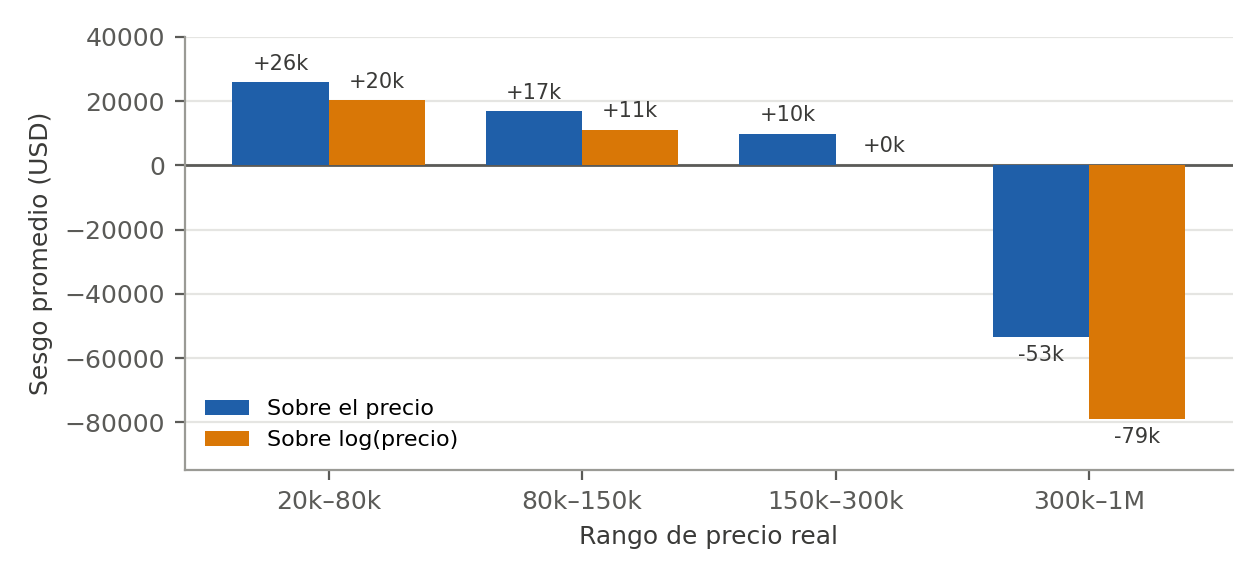
\includegraphics[width=0.89\linewidth]{media/figura4_sesgo_por_rango.png}
\caption*{Figura 4. Sesgo promedio por rango de precio. Valores positivos indican sobreestimación. La transformación logarítmica reduce el sesgo en los tres rangos inferiores y lo agrava en el superior.}
\end{figure}El sesgo baja de +25.918 a +20.426 dólares en el rango de 20.000 a 80.000, de +16.946 a +11.101 en el siguiente, y prácticamente desaparece entre 150.000 y 300.000 (+236). A cambio empeora en las propiedades de más de 300.000, de −53.353 a −78.957: al promediar en escala logarítmica y volver a dólares se obtiene algo cercano a la mediana, que queda por debajo de la media donde la cola es larga. Adoptamos el modelo logarítmico porque mejora el error relativo (24,9\% contra 27,1\%) y corrige el sesgo justamente en el rango donde opera esta inversora.

\textbf{Lo que ninguna de las dos métricas captura:} MAE y MAPE penalizan igual los errores por exceso y por defecto, mientras que para este problema sobreestimar es más caro. Un tratamiento completo usaría una pérdida asimétrica (por ejemplo, regresión cuantílica sobre un cuantil inferior) o aplicaría un margen de seguridad a la predicción antes de decidir. Queda fuera del alcance de un prototipo, pero la elección de métrica no es neutral respecto del problema.

\subsection*{2.6 Qué mira el modelo}

La importancia por permutación mide cuánto empeora el error al desordenar una variable: si el modelo no la usa, desordenarla no cambia nada.

\begin{longtable}[]{@{}
  >{\raggedright\arraybackslash}p{(\columnwidth - 2\tabcolsep) * \real{0.6000}}
  >{\raggedright\arraybackslash}p{(\columnwidth - 2\tabcolsep) * \real{0.4000}}@{}}
\toprule\noalign{}
\begin{minipage}[b]{\linewidth}\raggedright
\textbf{Variable}
\end{minipage} & \begin{minipage}[b]{\linewidth}\raggedright
\textbf{Aumento del MAE (escala log)}
\end{minipage} \\
\midrule\noalign{}
\endhead
\bottomrule\noalign{}
\endlastfoot
Superficie & 0,248 \\
Barrio (l3) & 0,169 \\
Baños & 0,118 \\
Ambientes & 0,020 \\
Tipo de propiedad & 0,016 \\
Dormitorios & 0,012 \\
Longitud / Latitud & 0,012 / 0,011 \\
Provincia (l2) & 0,001 \\
\end{longtable}

Superficie, barrio y baños concentran casi toda la capacidad predictiva, lo que coincide con el criterio que usaría un tasador. Las coordenadas aportan poco una vez que el barrio está presente, porque codifican la misma información de forma redundante, y la provincia es casi irrelevante por la misma razón. Que el modelo reproduzca el criterio del dominio, sin que se lo hayamos impuesto, es un indicio de que aprendió algo razonable.

\subsection*{2.7 De la predicción a la decisión}

Definimos como candidata a oportunidad el aviso cuyo precio publicado está más de 30\% por debajo del valor estimado. Sobre los 58.877 avisos del período de evaluación, el modelo marca 6.469, el 11\%: el filtro descarta nueve de cada diez propiedades sin necesidad de visitarlas, que es exactamente el valor operativo buscado.

Ahora bien, al inspeccionar las brechas más grandes aparecen casos como una casa de 1.060 m² publicada a 22.000 dólares o un departamento de 76 m² en Vicente López a 23.000. No son gangas: son avisos con datos mal cargados, o publicaciones donde el precio es un valor de referencia y no el real. Esto refuerza que la salida del modelo es una lista de prioridades para revisar, no una lista de compras, y que conviene descartar automáticamente las brechas extremas, que son casi siempre errores de carga antes que oportunidades.

\subsection*{2.8 Factibilidad operativa}

\textbf{Desafío 1 --- Los datos miden algo distinto de lo que queremos predecir.} Properati publica precios de oferta, no de transacción: el modelo aprende qué pide el vendedor, no qué pagó el comprador. En un mercado donde se negocia, ambos difieren y siempre en la misma dirección, de modo que el modelo sobreestima sistemáticamente el valor. Esa brecha está medida: Reporte Inmobiliario la publica mensualmente y en enero de 2026 fue de −5,14\%, el primer registro en 21 meses que supera el 5\% (venía de −4,92\% en noviembre). Para una inversora que compra, esa sobreestimación es precisamente el error caro.

El dato de cierre a nivel operación no está disponible ---las escrituras no son públicas y los registros publican agregados con rezago---, pero el agregado mensual sí lo está, y eso habilita una corrección concreta: descontar la brecha publicada de cada predicción y tratar el resultado como techo del valor, no como estimación central. Es un parche calibrado con una fuente externa, no un supuesto. A esto se suma el 37\% de avisos sin superficie informada, que el modelo directamente no puede evaluar.

\textbf{Desafío 2 --- El modelo se degrada y requiere monitoreo.} El error relativo crece de forma sostenida a lo largo del período de evaluación, a razón de unos 0,85 puntos porcentuales por mes.

\begin{figure}[H]
\centering
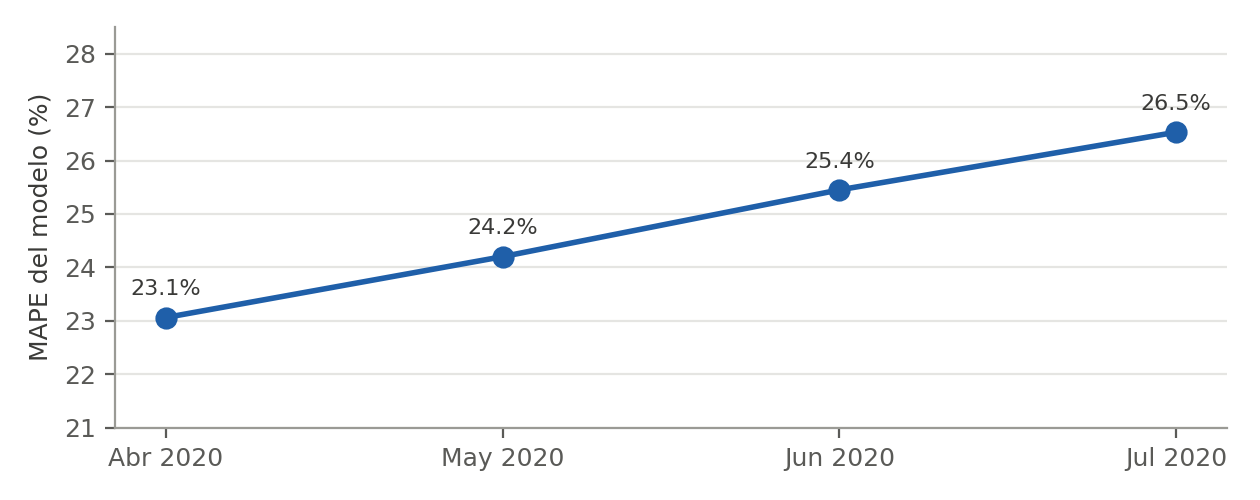
\includegraphics[width=0.86\linewidth]{media/figura5_error_por_mes.png}
\caption*{Figura 5. Error relativo del modelo por mes de publicación, sobre el conjunto de evaluación (abril a julio de 2020).}
\end{figure}Conviven los dos tipos de cambio que vimos en clase: cambió qué se publica (menos avisos, otro mix de propiedades y zonas), que es covariate shift, y cambió cuánto vale una misma propiedad con las mismas características, que es concept drift. Entendemos que domina el segundo, porque el valor de una vivienda depende de variables macroeconómicas que el modelo no observa ---tipo de cambio, crédito hipotecario disponible, expectativas--- y cuando esas se mueven, la relación entre características y precio se desplaza aunque el conjunto de propiedades publicadas sea el mismo.

La política que se desprende es reentrenar trimestralmente: con una degradación de 0,85 puntos por mes, un trimestre implica tolerar unos 2,5 puntos de MAPE, llevando el error del 25\% al 27,5\%. Es aceptable para priorizar visitas, un uso tolerante al error; no lo sería para fijar el precio de una operación. El monitoreo debe cubrir dos planos: la métrica sobre las propiedades efectivamente visitadas y con desenlace conocido, con alerta si el MAPE supera los 30 puntos, y la distribución de las variables de entrada, para detectar el covariate shift antes de que impacte en la métrica. Para lo primero alcanza con un reporte periódico; para lo segundo, herramientas de reglas sobre datos como Great Expectations, orquestadas junto con el reentrenamiento.

\textbf{Desafío 3 --- Costos y justificación económica.} Para evaluar si el sistema se paga hay que partir de la economía de una operación de flipping, con valores de mercado y no supuestos. Tomamos como unidad un departamento de dos ambientes en CABA, cuyo precio de publicación promedio era de USD 131.272 en agosto de 2026 (Zonaprop), con un m² promedio de USD 2.476.

\begin{longtable}[]{@{}
  >{\raggedright\arraybackslash}p{(\columnwidth - 4\tabcolsep) * \real{0.4200}}
  >{\raggedright\arraybackslash}p{(\columnwidth - 4\tabcolsep) * \real{0.3300}}
  >{\raggedright\arraybackslash}p{(\columnwidth - 4\tabcolsep) * \real{0.2500}}@{}}
\toprule\noalign{}
\begin{minipage}[b]{\linewidth}\raggedright
\textbf{Concepto}
\end{minipage} & \begin{minipage}[b]{\linewidth}\raggedright
\textbf{Fuente / criterio}
\end{minipage} & \begin{minipage}[b]{\linewidth}\raggedright
\textbf{Monto}
\end{minipage} \\
\midrule\noalign{}
\endhead
\bottomrule\noalign{}
\endlastfoot
Compra con 30\% por debajo del valor de mercado & Umbral que define una candidata & USD 91.890 \\
Gastos de compra (escribano, sellos, certificaciones): 6\% & La Nación, abril 2026 (rango 5\%--8\%) & USD 5.513 \\
Refacción media: baño, cocina y pintura & Reporte Inmobiliario, enero 2026 & USD 14.000 \\
Inversión total & & USD 111.403 \\
Venta a valor de mercado, neta de 5,5\% de gastos & Comisión 3--4\% más mitad del sellado & USD 124.052 \\
Margen por operación & & USD 12.649 \\
Operación del sistema (datos, cómputo, mantenimiento) & Estimación propia & USD 400 por mes \\
\end{longtable}

La cuenta deja dos conclusiones. La primera es que el margen real por operación ronda los USD 12.600, un 11\% sobre la inversión, bastante menos de lo que sugiere la intuición: los gastos de transacción y la refacción se llevan buena parte de la diferencia. La segunda es más interesante: si el descuento de compra fuera del 20\% en lugar del 30\%, la operación daría pérdida. El umbral del 30\% que usamos para marcar candidatas no es entonces un número arbitrario, sino aproximadamente el mínimo que hace viable el negocio, y eso le da sentido económico al filtro del modelo.

Contra ese margen, el costo del sistema es menor: USD 4.800 anuales, equivalentes al 38\% de una sola operación. Se paga de dos maneras alternativas, y con cualquiera alcanza: generando una operación adicional cada tres años, o evitando una sola compra sobrevaluada, dado que ignorar la brecha de negociación del 5,14\% sobre una propiedad de USD 131.272 implica pagar USD 6.747 de más, más de un año de costo del sistema.

La contracara es que ese beneficio supone que las candidatas son oportunidades reales. Si la proporción de falsos positivos fuera alta, el costo relevante no sería el del sistema sino el tiempo de la inversora, que es el recurso verdaderamente escaso: con ocho visitas mensuales sobre miles de avisos, cada visita desperdiciada tiene un costo de oportunidad alto. Medir esa proporción exige registrar el resultado de cada visita, lo que convierte al seguimiento en una inversión necesaria y no en un agregado opcional.

\section*{Conclusiones}

\begin{itemize}
\item
  En ambas partes, la mayor ganancia vino del trabajo sobre los datos y no de la elección del modelo: en Home Credit las variables construidas aportaron +0,018 de AUC contra +0,002 del tuning; en Properati, los límites del prototipo son de los datos disponibles, no del algoritmo.
\item
  Validar como se va a usar el modelo cambia las conclusiones: la partición temporal en la Parte 2 expuso una degradación que una partición aleatoria habría ocultado.
\item
  Interpretar no es un paso decorativo. En la Parte 1 reveló una variable predictiva pero éticamente problemática; en la Parte 2 mostró un sesgo sistemático que invertía el sentido de las oportunidades detectadas.
\item
  Las métricas estándar incorporan supuestos que conviene hacer explícitos: ni MAE ni MAPE distinguen sobreestimar de subestimar, aunque para el problema planteado una cosa cuesta mucho más que la otra.
\end{itemize}

\section*{Fuentes}

\begin{itemize}
\item
  Home Credit Default Risk, competencia y datos: kaggle.com/competitions/home-credit-default-risk
\item
  Properati Argentina Dataset: kaggle.com/datasets/alejandroczernikier/properati-argentina-dataset
\item
  Brecha entre precio de publicación y precio real de cierre (−5,14\%, enero 2026): Reporte Inmobiliario, ``Precio real de cierre por m²'', reporteinmobiliario.com
\item
  Precio promedio del m² y de unidades tipo en CABA (agosto 2026): informe de Zonaprop publicado el 8 de septiembre de 2026, mercado.com.ar
\item
  Costos de refacción por ambiente (enero 2026): Reporte Inmobiliario, reproducido en La Nación, ``Uno por uno: estos son los costos para hacer una remodelación'', 29 de marzo de 2026
\item
  Gastos de escrituración y comisiones en CABA: La Nación, ``Escritura de una propiedad: qué gastos hay que pagar'', abril de 2026
\end{itemize}

\section*{Anexo · Estructura del código}

\begin{longtable}[]{@{}
  >{\raggedright\arraybackslash}p{(\columnwidth - 2\tabcolsep) * \real{0.3300}}
  >{\raggedright\arraybackslash}p{(\columnwidth - 2\tabcolsep) * \real{0.6700}}@{}}
\toprule\noalign{}
\begin{minipage}[b]{\linewidth}\raggedright
\textbf{Archivo}
\end{minipage} & \begin{minipage}[b]{\linewidth}\raggedright
\textbf{Qué hace}
\end{minipage} \\
\midrule\noalign{}
\endhead
\bottomrule\noalign{}
\endlastfoot
src/features.py & Feature engineering de la Parte 1 (application, bureau, previous, installments) \\
src/features\_\allowbreak{}bureau.py & Features de bureau y bureau\_\allowbreak{}balance con agregación en dos niveles \\
src/eval\_\allowbreak{}bureau.py & Comparación de las variantes de bureau sobre los folds fijos \\
src/models.py & Logística baseline y LightGBM (categóricas nativas u one-hot) \\
src/cv.py & Validación cruzada con los folds fijos (OOF, AUC y predicción de test) \\
src/make\_\allowbreak{}folds.py & Genera y versiona la partición en 5 folds estratificados \\
src/tuning.py & Optimización de hiperparámetros con Optuna \\
src/interpretability.py & Importancia por ganancia y valores SHAP \\
src/parte2\_\allowbreak{}properati.py & Parte 2 completa: filtros, partición temporal, baseline, prototipo y diagnósticos \\
resultados/ y resultados\_\allowbreak{}parte2/ & Tablas y figuras que se citan en este informe \\
\end{longtable}


\end{document}
